\chapter{Appendix}

\section*{Resources and Links}

\begin{itemize}
    \item Dataset: \url{https://isip.piconepress.com/projects/nedc/html/tuh_eeg/}
    \item Braindecode: \url{https://braindecode.org/stable/index.html}
    \item GitHub: \url{https://github.com/BenjaminToth/MScThesis}
\end{itemize}

\section*{Example Synthetic EEG Artifact}

\begin{figure}[H]
\centering
    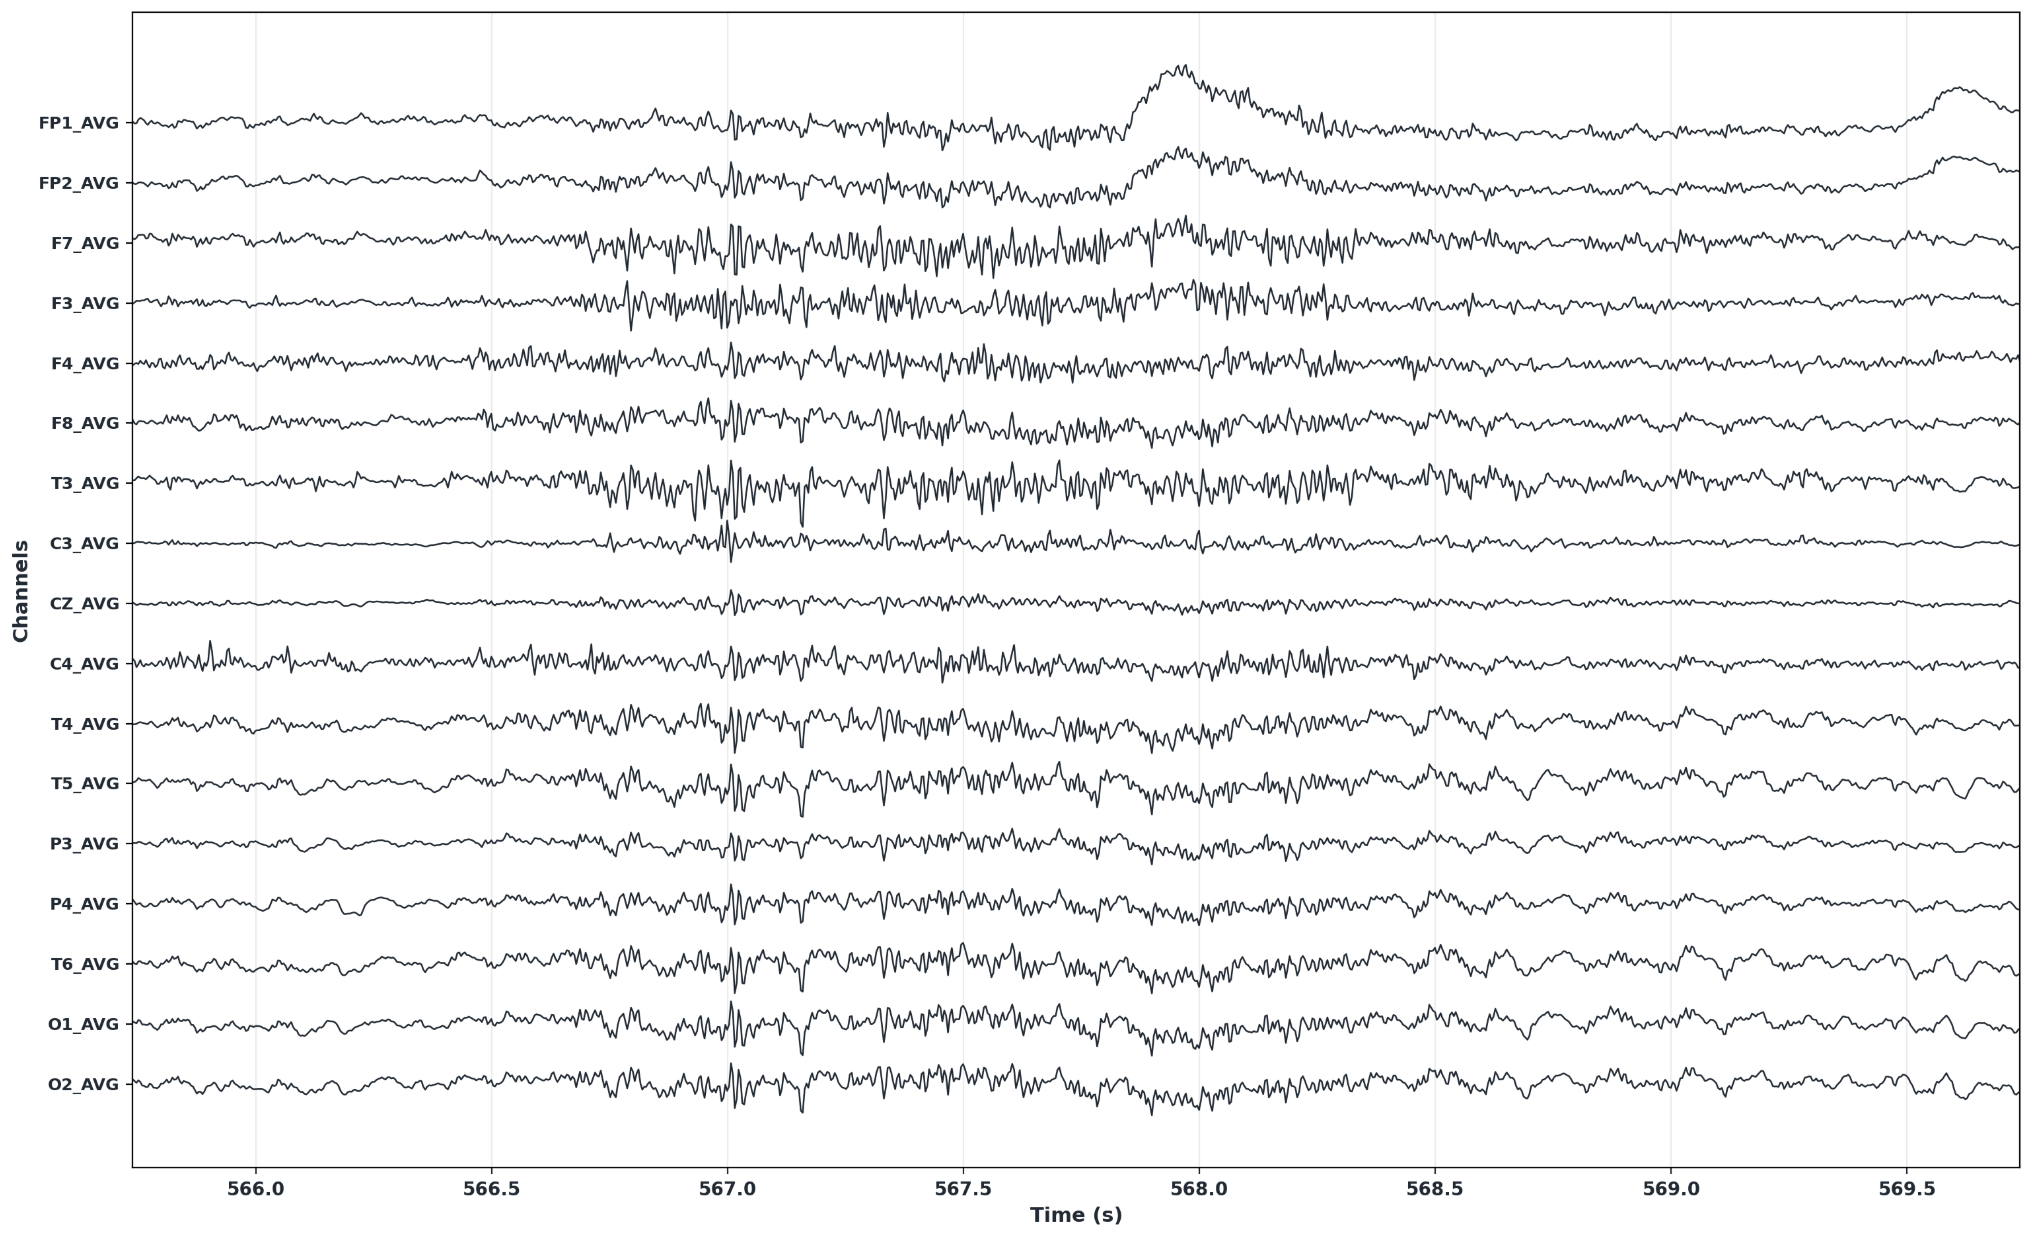
\includegraphics[width=1\textwidth]{images/synthetic_eyem.png}
    \caption{Example synthetic EEG window generated using the proposed latent diffusion-based augmentation method. For the generation the model corresponding to the eyem artifact was used.}
    \label{fig:eyem}
\end{figure}

\section*{Model Parameters}

The models are based on the original Braindecode implementation, with small modifications to better suit the requirements of this study.

All models were trained on EEG segments with $C=17$ channels and $T=2000$ time samples.

\paragraph{EEGNet}
\begin{itemize}
    \item Dropout $p=0.5$
    \item Kernel sizes: $k_t=63$, $k_d=15$
    \item Filters: $F_1=8$, depth multiplier $D=2$, $F_2=16$
\end{itemize}

\paragraph{EEGNeX}
\begin{itemize}
    \item Activation: ELU, dropout $p=0.5$
    \item Filters: $F_1=8$, $F_2=32$, $D=2$, $F_3=64$
    \item Kernel sizes: $k_{1,2}=32$, $k_4=16$, $k_5=16$
    \item Dilations: $d_4=2$, $d_5=4$
    \item Pooling: $p_4=4$, $p_5=8$
    \item Max-norm: conv $=1.0$, linear $=0.25$
\end{itemize}

\paragraph{EEGInceptionERP}
\begin{itemize}
    \item Activation: ELU, dropout $p=0.5$
    \item Base filters: $F=8$, depth multiplier $D=2$
    \item Stage 1 kernels: $(64, 32, 16)$
    \item Stage 2 kernels: $(16, 8, 4)$
    \item Stage 3--4 kernels: $k_3=8$, $k_4=4$
    \item Pooling: $p_1=4$, $p_2=2$, $p_3=2$, $p_4=2$
\end{itemize}

\paragraph{CNN-LSTM}
\begin{itemize}
    \item Activation: ELU, dropout $p=0.35$
    \item CNN filters: $F_1=64$, $F_2=128$
    \item Kernel sizes: $k_1=15$, $k_2=7$
    \item Pooling: $p_1=2$, $p_2=2$
    \item LSTM: hidden size $H=192$, layers $L=2$, bidirectional
\end{itemize}

\paragraph{EEGConformer}
\begin{itemize}
    \item Embedding size: $D=40$
    \item Temporal kernel: $k_t=25$
    \item Patch pooling: kernel $=75$, stride $=15$
    \item Transformer: depth $L=6$, heads $H=10$
    \item Feed-forward expansion: $4$
    \item Classification head: hidden size $256$
    \item Activations: ELU (front-end), GELU (transformer)
    \item Dropout: $p=0.5$, attention dropout $p_{\text{att}}=0.5$
\end{itemize}

\paragraph{WGAN-GP}
\begin{itemize}
    \item Input/output shape: $C=17$, $T=2000$
    \item Latent dimension: $z=128$
    \item Generator base channels: $256$
    \item Generator channel progression: $256 \rightarrow 256 \rightarrow 128 \rightarrow 64 \rightarrow 32 \rightarrow 17$
    \item Generator kernel sizes: $k=5$ (hidden), $k_{\text{out}}=7$
    \item Generator normalization: GroupNorm, activation: LeakyReLU$(0.2)$
    \item Critic channels: $64 \rightarrow 128 \rightarrow 256 \rightarrow 512$
    \item Critic kernel size: $k=5$, stride $s=2$, pooling length $16$
    \item Gradient penalty: $\lambda_{\mathrm{gp}}=10$
    \item Training ratio: $n_{\text{critic}}=5$
    \item Optimizer: Adam, $\mathrm{lr}_G=\mathrm{lr}_D=2 \times 10^{-4}$, $\beta_1=0.0$, $\beta_2=0.9$
\end{itemize}

\paragraph{Latent Diffusion Model}
\begin{itemize}
    \item Input/output shape: $C=17$, $T=2000$
    \item Latent shape: $C_z=32$, $T_z=125$
    \item VAE: base channels $F=128$, downsampling factor $16$, kernel sizes $k=5$ (encoder/decoder), $k_{\mathrm{out}}=7$, activation SiLU, GroupNorm
    \item Latent U-Net: base channels $F=128$, channel multipliers $(1,2,4)$, residual block kernel size $k=3$, downsampling kernel $k=4$ with stride $s=2$, bottleneck blocks $=2$
    \item Time embedding: sinusoidal, dimension $D_t=256$, MLP expansion $4\times$
    \item Diffusion: timesteps $N=1000$, beta schedule cosine, inference steps $50$
    \item Training: VAE epochs $10$, diffusion epochs $20$, batch size $32$, gradient clipping $1.0$
    \item Optimisation: Adam, $\mathrm{lr}_{\mathrm{VAE}}=10^{-3}$, $\mathrm{lr}_{\mathrm{diff}}=2 \times 10^{-4}$
    \item VAE objective: reconstruction loss $L_1$, KL weight $\lambda_{\mathrm{KL}}=10^{-4}$
    \item Latent scaling: auto-estimated to approximately unit variance
\end{itemize}

\newpage

\subsubsection{Use of AI Tools and Figure Attribution:}

All architecture images were created by the author.

AI tools were used to improve the grammar and vocabulary of most parts of this thesis in order to achieve an appropriate academic style. All AI-generated suggestions were carefully reviewed and either revised or discarded as necessary.

The code in the accompanying repository was developed with the assistance of AI tools. These tools were used for tasks such as error handling, visualisation, README refinement, implementation of helper functions, as well as code optimisation and refactoring. AI assistance also contributed to the fine-tuning of model architectures from braindecode. All AI-generated code and suggestions were carefully reviewed and, where necessary, modified or rejected by the author.

The preprocessing pipeline and data loaders were developed with the help of, and based on, the work of the AI Research Group at the Institute of Mathematics, Eötvös Loránd University.
